\section{Approach} \label{Sec:approach}
At high level, our approach generates function level assertions for the \javascript code by utilizing human written DOM-based tests and assertions. Our code level assertions fall in the following three categories: (1) explicit assertions, which are directly inferred from analyzing the manually written DOM-based assertions, (2) implicit assertions, which are indirectly connected to human written DOM-based assertions, and (3) potential candidate assertions, which are not included in the written DOM-based assertions, yet are potentially useful to be checked by the function level test suite. We discuss each of the aforementioned categories in the following subsections in more details.
\IncMargin{0em}
\begin{algorithm}[t]
{\scriptsize
\SetKwInOut{Input}{input}\SetKwInOut{Output}{output}
\Input{Test suite $T$; The set of test cases $tc_i \in T$}
\Output{The ordered set of oracles $oracles$}
\BlankLine

\Begin {
\nl \For{$tc_i \in T$}{
\nl  $trace \leftarrow textsc{Exec}(tc_i)$\\
\nl  $domAccss \leftarrow \textsc{GetDOMAcc}(trace)$\\   	
\nl  $freqAccdDOM\leftarrow \emptyset$\\
\nl  \For{$dom \in domAccss $}{
\nl   \If{$\textsc{DOMUsgFreq}(dom) \geq \frac{1}{NoOfDOMElems} $}{
\nl    $freqAccdDOM \leftarrow dom \cup freqAccdDOM$\\       
      }
     }
\nl  \For{$asstn \in assertions_{tc_i}$}{
\nl   $asserDOMAcc \leftarrow \textsc{GetDOMAcc}(asstn)$\\
\nl   $asserDOMMuts \leftarrow \textsc{GetDOMMuts}(asserDOMAcc)$\\
\nl   \For{$domMut \in asserDOMMuts$}{
\nl    $bwSts \leftarrow \textsc{GetBWSlice}(domMut, trace)$\\
\nl    $asstnRel \leftarrow \textsc{GetWrVars}(bwSts)$\\
\nl    $potAsstnRel \leftarrow \textsc{GetFWSlice}(asstnRel, trace)$\\
      }
     }
\nl  $nonAsserDOMMuts \leftarrow \textsc{GetDOMMuts}(freqAccdDOM)$\\
\nl  \For{$domMut \in nonAsserDOMMuts$}{
\nl   $bwSts \leftarrow \textsc{GetBWSlice}(domMut, trace)$\\
\nl   $nonAsstnRel \leftarrow \textsc{GetWrVars}(bwSts)$\\
     }
\nl  $asstnRelOrcls[func]_{f=1}^{n} \leftarrow \textsc{GetValue}(\textsc{Accessibles}([func]_{f=1}^{n}, asstnRel))$\\
\nl  $candidOrcls[func]_{f=1}^{n} \leftarrow \textsc{Accessibles}([func]_{f=1}^{n}, [potAsstnRel \cup nonAsstnRel])$\\
\nl  $oracles[func]_{f=1}^{n}.\textsc{Add}(asstnRelOrcls \cup candidOrcls)$\\
   }
\nl $\textsc{Rank}(oracles[func]_{f=1}^{n})$\\
\nl return $(oracles[func]_{f=1}^{n})$
}
\caption{Oracle Generation} 
\label{Alg:algorithm}
}
\end{algorithm}
%\DecMargin{lem}
\begin{figure*}
  \centering
  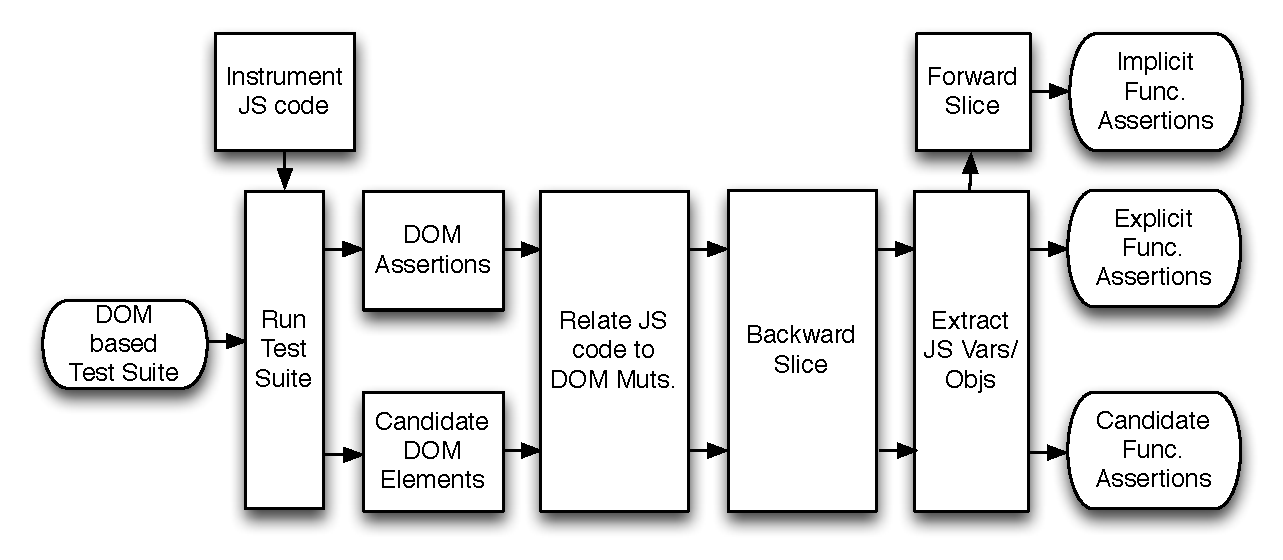
\includegraphics[width=.7\hsize]{fig/approachDiagram}
  \mycaption{Overview of our assertion generation approach.}
  \vspace{-0.1in} 
  \label{Fig:approachDiagram}
  \vspace{-0.1in} 
\end{figure*}
%mutation of customer.couponStatus = coupon.Id + '-' + 'used' to customer.couponStatus = coupon.Id + 'used';'